\documentclass[../main.tex]{subfiles}
\begin{document}
Le espressioni regolari permetto di cercare delle sequenze di caratteri all'interno di stringhe di testo. Fino ad ora abbiamo visto ad
esempio il comando \code{grep}, tuttavia è piuttosto limitato. Per testare utilizzare il sito \code{regex101}.

\subsection{Pattern semplici}
\begin{itemize}
    \item \textbf{Singoli caratteri: } \code{b}, cerca il carattere b all'interno del testo
    \item \textbf{Sequenze di più caratteri: }, \code{mani} cerca la sequenza mani all'interno del testo (mani, romani, umani, ...)
\end{itemize}

\subsection{Caratteri speciali}
Alcuni caratteri assumono un significato speciale se sono preceduti da \code{\textbackslash}:
\begin{figure}[h]
    \centering
    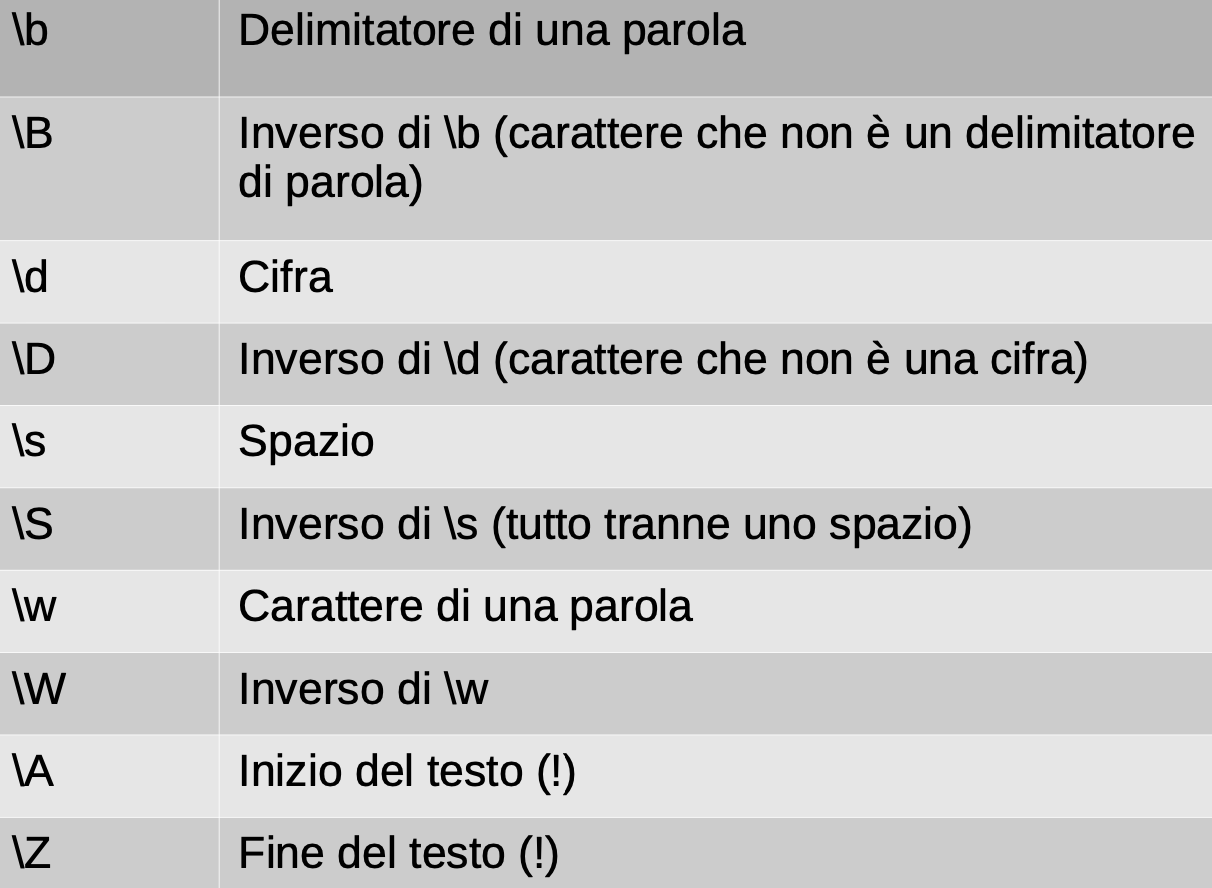
\includegraphics[width=0.5\textwidth]{../images/caratteriRegExp.png}
\end{figure}

\vspace{0.25cm}
Altri sono speciali senza l'utilizzo del \code{\textbackslash}:
\begin{figure}[h]
    \centering
    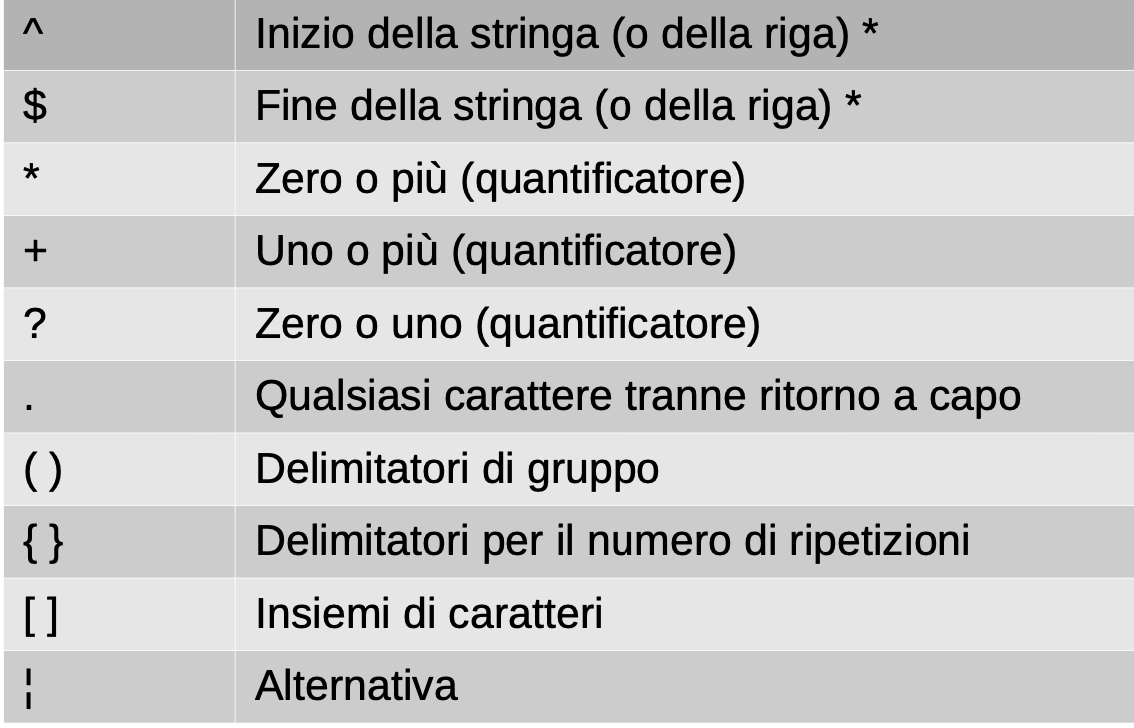
\includegraphics[width=0.5\textwidth]{../images/caratteriSpeciali.png}
\end{figure}

\textbf{Nota:} per trovare il carattere effettivo bisogna mettere prima \code{\textbackslash}, ad esempio \code{\textbackslash*}.

\vspace{0.5cm}
\subsubsection{Alternative}
Trova \code{ciao} oppure \code{cibo}, inoltre crea dei sottomatch per \code{ia} e \code{ib}.
\begin{lstlisting}[style=bash]
    c(ia | ib)o
\end{lstlisting}

\pagebreak
\subsection{Esempi}
Di base per cercare con le \code{regexp} usiamo \code{grep -E "regexp" a.txt}.

\begin{itemize}
    \item Trovare tutte le parole di un testo potremmo usare
    \begin{lstlisting}[style=bash]
        \b[A-Za-z]+\b
    
        #oppure
    
        \b[[:alpha:]]+\b
    \end{lstlisting}
    \item Trovare tutte le parole palindrome di quattro lettere
    \begin{lstlisting}[style=bash]
        \b(\w)(\w)\2\1\b
    \end{lstlisting}
\end{itemize}

\vspace{1cm}
\subsection{\code{grep}}
\begin{lstlisting}[style=bash]
    grep -E "\bmani\b" testo.txt
\end{lstlisting}
%Tabella slide 5

\vspace{1cm}
\subsection{\code{sed}}
\begin{itemize}
    \item Modifica un flusso di caratteri
    \item Lavora riga per riga
\end{itemize}
\begin{lstlisting}[style=bash]
    sed [opzioni] -e 'espressione' inputfile
\end{lstlisting}
%Tabella slide 9

\vspace{0.5cm}
\subsubsection{\code{s///}}
\begin{itemize}
    \item Utilizzare \code{sed} per ostituire un termine con un altro
    \item \code{g} Sostituisce tutte le corrispondenze della riga (non solo la prima corrispondenza per ogni riga)
    \item \code{I} rende il comando case insensitive
\end{itemize}
\begin{lstlisting}[style=bash]
    sed -E -e 's/\bmani\b/piedi/' testo.txt
\end{lstlisting}

\vspace{0.5cm}
\begin{itemize}
    \item Con \code{\&} Posso utilizzare il valore dell'espressione regolare
\end{itemize}
\begin{lstlisting}[style=bash]
    #testo.txt contiene: ciao come stai

    sed -E -e 's/.*/Linea: &/g' testo.txt

    #OUTPUT: Linea: ciao come stai
\end{lstlisting}

\vspace{0.5cm}
\begin{itemize}
    \item Posso referenziare i gruppi usati con la notazione \code{\textbackslash N}
\end{itemize}
\begin{lstlisting}[style=bash]
    sed -E -e 's/(\w)(\w)/\2\1/g' testo.txt
\end{lstlisting}

\pagebreak
\begin{itemize}
    \item Posso specificare una singola riga o un intervallo di righe sulla quale cercare le corrispondenze (indirizzo)
\end{itemize}
\begin{lstlisting}[style=bash]
    #Da riga 2 a riga 3
    sed -E -e '2,3 s/(\w)(\w)/\2\1/g' testo.txt

    #In questo caso l'indirizzo è un espressione regolare
    sed -E -e '/\bmani\b/ s/(\w)(\w)/\2\1/g' testo.txt

    #Dalla riga 1 fino alla parola 'mani'
    sed -E -e '1,/\bmani\b/ s/(\w)(\w)/\2\1/g' testo.txt
\end{lstlisting}
\begin{figure}[h]
    \centering
    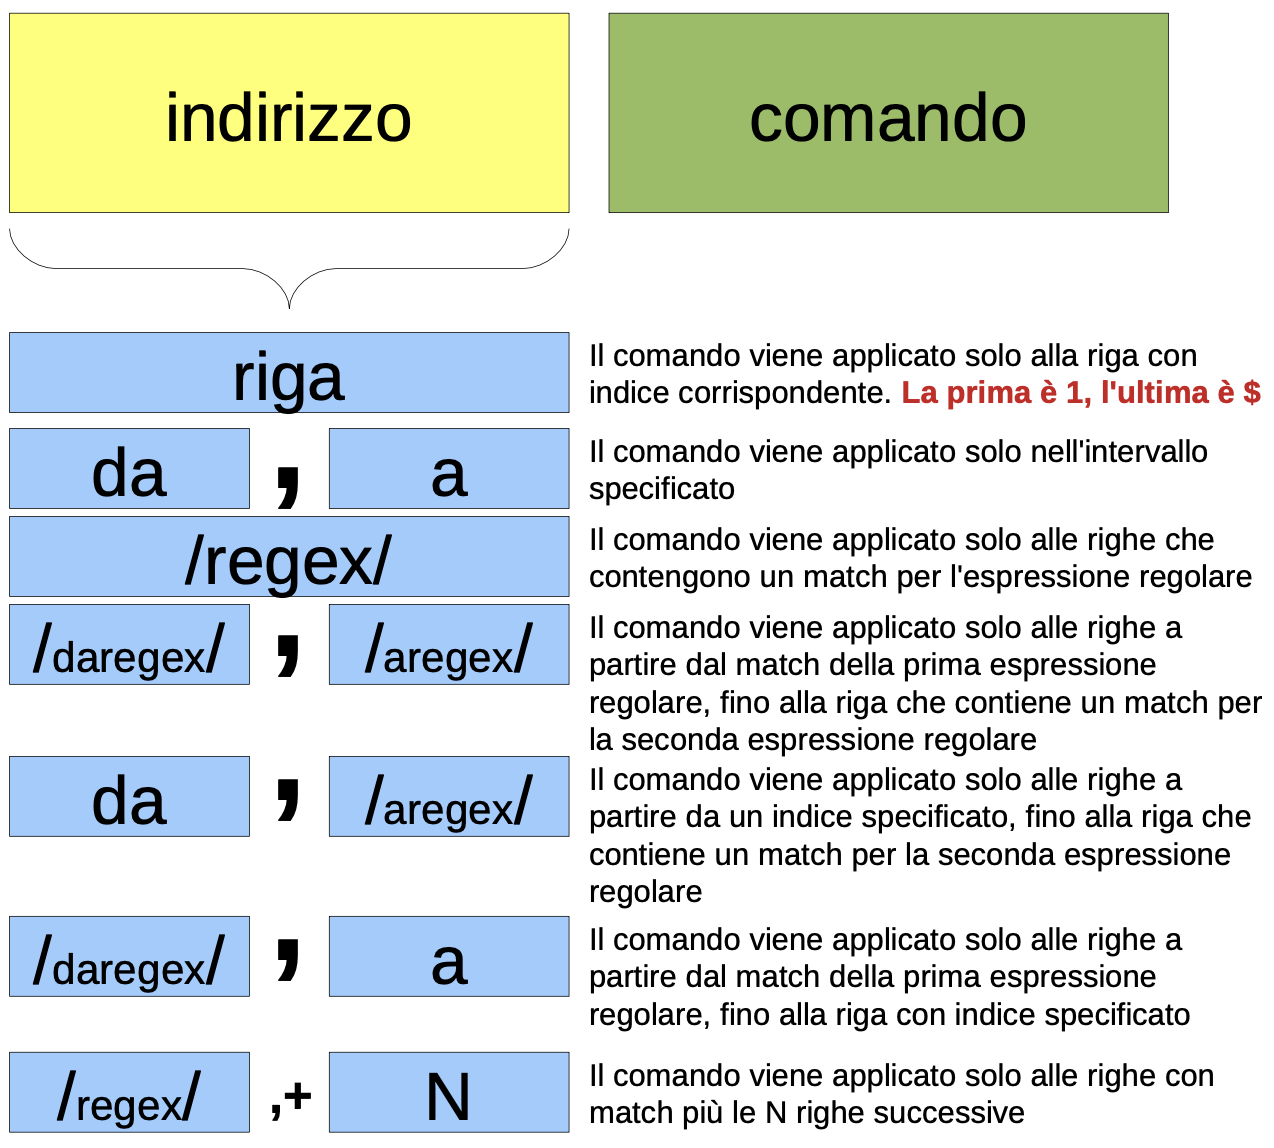
\includegraphics[width=0.5\textwidth]{../images/sep.png}
\end{figure}


\vspace{1cm}
\begin{itemize}
    \item Se aggiungo \code{!} all'indirizzo posso invertire le corrispondenze
\end{itemize}
\begin{lstlisting}[style=bash]
    #Stampa le righe che NON contengono le
    sed -E -n -e '/le/!p' testo.txt
\end{lstlisting}

\vspace{0.5cm}
\begin{itemize}
    \item Posso stampare tutte le righe che contengono una parola
\end{itemize}
\begin{lstlisting}[style=bash]
    #Stampa le righe 1 e 3
    sed -E -n -e '1,3p' testo.txt
\end{lstlisting}

\vspace{0.5cm}
\begin{itemize}
    \item Posso cancellare determinate righe
\end{itemize}
\begin{lstlisting}[style=bash]
    #Cancella le righe 1 e 2
    sed -E '1,3d' testo.txt
\end{lstlisting}

\vspace{0.5cm}
\begin{itemize}
    \item Posso effettuare sostituzioni tra due gruppi di caratteri (di lunghezza uguale), carattere per carattere
\end{itemize}
\begin{lstlisting}[style=bash]
    #Sostituisce la s con 5, la l con 1, la e con 3 e la o con 0
    sed -E -e 'y/sleo/5130/' testo.txt
\end{lstlisting}

\pagebreak
\begin{itemize}
    \item Posso inserire una o più righe prima o dopo di ogni riga
\end{itemize}
\begin{lstlisting}[style=bash]
    #Aggiunge una riga "Riga aggiuntiva" e una riga "Altra riga" prima della riga dalla riva 1 alla riga 3
    sed -E -e "1,3iRiga aggiunta\nAltra riga" testo.txt

    #Aggiunge una riga "Riga aggiuntiva" e una riga "Altra riga" dopo alla riga dalla riva 1 alla riga 3
    sed -E -e "1,3aRiga aggiunta\nAltra riga" testo.txt
\end{lstlisting}

\vspace{0.5cm}
\begin{itemize}
    \item Posso stampare i numeri di linea
\end{itemize}
\begin{lstlisting}[style=bash]
    #Stampa il numero di linea prima di ogni linea
    sed -E -e '=' testo.txt
\end{lstlisting}

\vspace{0.5cm}
\begin{itemize}
    \item Posso utilizzare qualsiasi delimitatore custom (oltre al carattere \$)
\end{itemize}
\begin{lstlisting}[style=bash]
    sed -E -e 's@c@a@g' testo.txt
\end{lstlisting}

\end{document}